\subsection{Error State Kalman Filter}
\subsubsection{Concept and Motivation}
While the Extended Kalman Filter provides a powerful framework for nonlinear estimation, it still linearizes directly around the full nominal state. For systems such as the INS, where the state includes both position, velocity, and attitude (represented by quaternions), this approach can lead to numerical inconsistencies, unstable orientation updates, and loss of orthogonality in rotation representations.  
\\ \\
To address these issues, the Error State Kalman Filter (ESKF) reformulates the estimation problem by separating the system into two parts, a \textit{``nominal state''} $\mathbf{x}$ and a \textit{``small error state''} $\delta\mathbf{x}$. The nominal state follows the nonlinear dynamics of the INS, while the error state captures small deviations from this nominal trajectory. This approach allows the filter to maintain accurate nonlinear propagation of the nominal state while estimating only small, approximately linear error quantities. 



\subsubsection{Error State Formulation}
The nominal INS model is already defined earlier in this work in Equation \ref{eq:kinematics-motion-model} with nominal states Equation \ref{eq:kinematics-motion-model-states}.
\\ \\
From the nominal INS model, the corresponding error state INS model is obtained by linearizing the nonlinear equations around the current nominal trajectory. This process isolates the small deviations between the true state and the estimated nominal state, allowing the linearized error dynamics to be described by a 1st order system. Following the formulation by Edmund Brekke in \textit{``Fundamentals of Sensor Fusion''} \cite{sensor_fusion_book}, the continuous time linear time varying (LTV) error state dynamics are expressed as
$$
    \delta\mathbf{x} =
    \begin{bmatrix}
        \delta\mathbf{p}_{b/O}^{n} \\
        \delta\mathbf{v}_{b/O}^{n} \\
        \delta\mathbf{\theta} \\
        \delta\mathbf{a}_b \\
        \delta\mathbf{\omega}_b
    \end{bmatrix}
$$
$$
    \delta\dot{\mathbf{x}} = A(\mathbf{x}) \, \delta\mathbf{x} + G(\mathbf{x})\,\mathbf{n}
$$
Here, $\delta\mathbf{x}$ represents the small deviation between the true and nominal state vectors, and $\mathbf{n}$ is the continuous time process noise, typically modeled as zero mean Gaussian white noise. The system matrices $A(\mathbf{x})$ and $G(\mathbf{x})$ depend on the current nominal state and describe how these small deviations evolve in time.  
\\ \\
The attitude error is represented using the small angle quaternion approximation, which linearizes the rotation error between the estimated and true attitudes. This approximation holds for small orientation deviations and is expressed as
$$
    \delta\mathbf{q} \approx
    \begin{bmatrix}
        1 \\
        \tfrac{\delta\boldsymbol{\theta}}{2}
    \end{bmatrix}
$$
This relation ensures that the attitude error $\delta\boldsymbol{\theta}$ can be treated as a 3D vector in the local tangent space of the unit quaternion manifold, simplifying the linearization of rotational dynamics while maintaining geometric consistency.  



\subsubsection{Process Model and Jacobians}
The linearized system matrices $A(\mathbf{x})$ and $G(\mathbf{x})$ are given by
$$
    A(\mathbf{x}) =
    \begin{bmatrix}
        \mathbf{0} & \mathbf{I} & \mathbf{0} & \mathbf{0} & \mathbf{0} \\
        \mathbf{0} & \mathbf{0} & -R_b^n(\mathbf{q})\,[\mathbf{a}_m - \mathbf{a}_{b}]_\times & -R_b^n(\mathbf{q}) & \mathbf{0} \\
        \mathbf{0} & \mathbf{0} & -[\boldsymbol{\omega}_m - \mathbf{\omega}_b]_\times & \mathbf{0} & -\mathbf{I} \\
        \mathbf{0} & \mathbf{0} & \mathbf{0} & \mathbf{-p_{\mathbf{a}b}\,I} & \mathbf{0} \\
        \mathbf{0} & \mathbf{0} & \mathbf{0} & \mathbf{0} & \mathbf{-p_{\mathbf{\omega}b}\,I}
    \end{bmatrix},
    \qquad
    G(\mathbf{x}) =
    \begin{bmatrix}
        \mathbf{0} & \mathbf{0} & \mathbf{0} & \mathbf{0} \\
        \mathbf{-R_b^n(\mathbf{q})} & \mathbf{0} & \mathbf{0} & \mathbf{0} \\
        \mathbf{0} & \mathbf{-I} & \mathbf{0} & \mathbf{0} \\
        \mathbf{0} & \mathbf{0} & \mathbf{I} & \mathbf{0} \\
        \mathbf{0} & \mathbf{0} & \mathbf{0} & \mathbf{I}
    \end{bmatrix}
$$
In this representation, $R_b^n(\mathbf{q})$ is the rotation matrix from the body frame to the navigation frame obtained from the current quaternion estimate $\mathbf{q}$. The notation $[\cdot]_\times$ denotes the skew-symmetric operator, which converts a 3D vector into a matrix form representing the cross product.  
\\ \\
The matrix $A(\mathbf{x})$ captures how small perturbations in position, velocity, attitude, and sensor biases evolve over time. The upper rows model the kinematic coupling between position and velocity, while the middle rows describe how accelerometer and gyroscope bias errors influence the navigation solution through attitude and velocity. The matrix $G(\mathbf{x})$ maps the continuous time process noise into the error dynamics, distributing the effect of IMU sensor noise, bias noise, and other stochastic disturbances into their corresponding error states.  
\\ \\
This linearized form provides the foundation for propagating the error state covariance in the ESKF. It allows the nonlinear nominal INS to run independently, while the filter maintains a linear and well behaved model of how uncertainty evolves, a key advantage that improves both numerical stability and estimation consistency.



\subsubsection{Discretization of Error Dynamics}
Discretization of the continuous error dynamics is critical for digital implementation. In theory, the discrete time transition matrix is given by
$$
    F_k = e^{A(\mathbf{x})\Delta t}, \qquad
    Q_k = \int_0^{\Delta t} e^{A(\mathbf{x})\tau} G(\mathbf{x}) Q G(\mathbf{x})^\top e^{A(\mathbf{x})^\top\tau} d\tau
$$
However, directly computing these expressions is infeasible in real-time embedded systems due to the computational cost of evaluating the matrix exponential and noise covariance integral at every time step. Several discretization strategies exist to approximate this process efficiently while maintaining filter stability and accuracy.  
\\ \\
The \textit{``Cayley'Hamilton series''} offers an exact polynomial expansion of the matrix exponential using the characteristic polynomial of $A(\mathbf{x})$. This approach is mathematically elegant and often employed for symbolic or algebraic analysis, particularly in time varying systems where analytic expressions for $A(\mathbf{x})$ are desired. However, in practical implementations, this method is highly inefficient. The repeated evaluation of high order polynomial terms and matrix powers makes it unsuitable for real-time embedded estimation where deterministic computational performance is required.  
\\ \\
A more practical and robust method is the ZOH discretization, introduced previously in Equation \ref{eq:ZOH}. The ZOH assumes that both the control inputs and process noise remain constant within each sampling interval. Under this assumption, it preserves the exact dynamics of linear time invariant systems and ensures numerical stability of the discrete time model. In practice, the ZOH discretization is implemented using an augmented matrix exponential containing the continuous time system matrices $A(\mathbf{x})$ and $G(\mathbf{x})$, which yields the discrete time transition matrix $F_k$ and the process noise covariance $Q_k$. This approach provides an accurate mapping from the continuous error dynamics to their discrete time equivalent while avoiding the instability of low order approximations.  
\\ \\
While theoretically precise, the ZOH can still be computationally demanding for real-time embedded systems, especially when matrix dimensions are large or $A(\mathbf{x})$ varies significantly over time. To address this, the \textit{``Padé approximation with scaling and squaring''}, defined in Equations \ref{eq:pade1}-\ref{eq:pade3}, is used in this work to efficiently approximate the matrix exponential. The Padé method offers an excellent trade off between numerical accuracy and computational speed. It remains stable even for ill conditioned matrices and maintains consistent results across varying sampling periods. This combination of ZOH based discretization and Padé based exponential approximation forms the foundation for robust real-time implementation of the ESKF.  
\\ \\
Finally, it is important to emphasize that crude 1st order approximations, such as assuming $F_k \approx I + A(\mathbf{x})\Delta t$, should be strictly avoided. Although computationally inexpensive, these approximations can introduce significant numerical errors, degrade covariance consistency, and cause filter divergence under high dynamic motion or long sampling intervals.



\subsubsection{Measurement Model and Jacobian}
Before defining the discrete time ESKF stages, the measurement Jacobian structure must be introduced. The total Jacobian used in the update step is expressed as
$$
    H = H_{\mathbf{x}} \, X_{\delta \mathbf{x}}.
$$
Here, $H_{\mathbf{x}}$ is the Jacobian of the measurement function with respect to the nominal state, obtained by linearizing the measurement model in Equation \ref{eq:aiding-measurement-model}. Since this measurement function provides position and yaw observations, $H_{\mathbf{x}}$ captures how small variations in the nominal position and attitude affect the predicted GNSS position and yaw outputs.  
\\ \\
However, because the ESKF performs estimation in the error state domain, the measurement sensitivity must be expressed with respect to the error state $\delta\mathbf{x}$. The matrix $X_{\delta \mathbf{x}}$ provides this mapping by relating perturbations in the nominal state to those in the error state. It has a fixed block diagonal structure:
$$
    X_{\delta \mathbf{x}} =
    \begin{bmatrix}
        I_6 & 0 & 0 \\
        0 & Q_{\delta\boldsymbol{\theta}} & 0 \\
        0 & 0 & I_6
    \end{bmatrix}
$$
where $Q_{\delta\boldsymbol{\theta}}$ relates small attitude errors $\delta\boldsymbol{\theta}$ to quaternion perturbations and is derived from the differential of $\mathbf{q} \otimes \delta\mathbf{q}$ evaluated at $\delta\boldsymbol{\theta}=0$, where $\mathbf{q} = [\eta \, \epsilon_1 \, \epsilon_2 \, \epsilon_3]^T$:
$$
    Q_{\delta\theta} \approx
    \frac{1}{2}
    \begin{bmatrix}
        -\epsilon_1 & -\epsilon_2 & -\epsilon_3 \\
         \eta & -\epsilon_3 & \epsilon_2 \\
         \epsilon_3 & \eta & -\epsilon_1 \\
        -\epsilon_2 & \epsilon_1 & \eta
    \end{bmatrix}.
$$
Together, $H_x$ and $X_{\delta x}$ form the complete measurement Jacobian $H = H_x X_{\delta x}$, which links measurement residuals to the linearized error state and enables consistent correction of both translational and rotational components during the update phase of the ESKF.



\subsubsection{Filter Algorithm}
The ESKF estimation process consists of several distinct stages, each responsible for different aspects of the nominal and error state propagation. The filter propagates the nonlinear nominal state using the INS equations, while maintaining a linearized covariance model of the small error dynamics. Unlike the EKF, the ESKF does not directly propagate the error-state mean, as it is always reset to zero after each correction. Instead, only the nominal state and the error covariance are propagated during the prediction stage.
\\ \\
\textbf{Prediction step:} \\ \noindent
At the beginning of each iteration, the error state mean is initialized to zero:
$$
    \delta\hat{\mathbf{x}}_{k|k-1} = \mathbf{0}
$$
The nominal state is propagated through the nonlinear discrete time INS process model:
$$
    \hat{\mathbf{x}}_{k|k-1} = f_d(\hat{\mathbf{x}}_{k-1|k-1}, \mathbf{u}_{k-1})
$$
Simultaneously, the covariance of the error state is propagated using the linearized system matrices $F_k$ and $Q_k$, derived from the Jacobians of the continuous time error dynamics:
$$
    P_{k|k-1} = F_k P_{k-1|k-1} F_k^\top + Q_k
$$
This step predicts the evolution of uncertainty around the nominal trajectory, incorporating the effects of process and sensor noise. The mean of the error state remains zero since the nominal state already represents the best estimate of the system.
\\ \\
\textbf{Update step:} \\ \noindent
When a new measurement $\mathbf{z}_k$ becomes available, the error state is updated using the linearized measurement model:
$$
\begin{aligned}
    K &= P_{k|k-1} H^\top (H P_{k|k-1} H^\top + R)^{-1} \\
    \delta\hat{\mathbf{x}}_{k|k} &= K [\mathbf{z}_k - h(\hat{\mathbf{x}}_{k|k-1})] \\
    P_{k|k} &= (I - K H) P_{k|k-1}
\end{aligned}
$$
Here, $H$ denotes the Jacobian of the measurement function with respect to the error state. The correction term $\delta\hat{\mathbf{x}}_{k|k}$ represents a small estimated deviation between the predicted nominal state and the measurement-derived state.
\\ \\
\textbf{Injection step:} \\ \noindent
After computing the correction, it is injected back into the nominal state using the nonlinear composition operator $\oplus$, which updates the nominal quantities according to the estimated error:
$$
    \hat{\mathbf{x}}_{k|k} \leftarrow \hat{\mathbf{x}}_{k|k-1} \oplus \delta\hat{\mathbf{x}}_{k|k}
$$
For translational states, this operation corresponds to vector addition, whereas for attitude states represented by quaternions, it involves quaternion multiplication between the nominal quaternion and the small-angle correction quaternion derived from $\delta\boldsymbol{\theta}$.
\\ \\
\textbf{Reset step:} \\ \noindent
Following the injection, the error state mean is reset to zero:
$$
    \delta\hat{\mathbf{x}}_{k|k} \leftarrow 0
$$
To maintain a consistent uncertainty representation after the nominal state update, the covariance must be transformed using the reset Jacobian $G$:
$$
    P_{k|k} \leftarrow G P_{k|k} G^\top, \qquad 
    G =
    \begin{bmatrix}
        I_6 & 0 & 0 \\
        0 & I - [\tfrac{\delta\hat{\boldsymbol{\theta}}}{2}]_\times & 0 \\
        0 & 0 & I_6
    \end{bmatrix}
$$
Here, $S = [\tfrac{\delta\hat{\boldsymbol{\theta}}}{2}]_\times$ denotes the small angle correction matrix related to the attitude quaternion update. This transformation ensures that the new error state is correctly defined relative to the updated nominal trajectory and that the covariance remains properly aligned, preventing the accumulation of linearization errors over time.
\\ \\
\textbf{Quaternion normalization:} \\ \noindent
Finally, quaternion normalization is applied to maintain a valid unit quaternion representation:
$$
    \mathbf{q}_{k|k} \leftarrow \frac{\mathbf{q}_{k|k}}{\|\mathbf{q}_{k|k}\|}
$$
This step guarantees that the attitude estimate remains on the unit hypersphere, preventing numerical drift and preserving a consistent rotation representation.
\\ \\
The combined structure of the prediction, update, injection, and reset stages allows the ESKF to maintain high numerical stability and consistency. By separating the nonlinear nominal state from the small linear error state, the filter achieves superior accuracy and robustness for inertial navigation systems involving rotational dynamics compared to the standard EKF formulation.



\subsubsection{EKF vs ESKF}
Overall, the ESKF provides significantly improved numerical stability, robustness, and estimation consistency compared to the EKF. By estimating only small, locally linear error quantities while maintaining a nonlinear nominal state propagation, it achieves an effective balance between accuracy and computational efficiency. This separation ensures that orientation updates remain well conditioned and free from singularities, even during highly dynamic motion. As a result, the ESKF has become the preferred framework for modern inertial navigation and sensor fusion systems, particularly in applications involving rotational dynamics and quaternion based attitude estimation.
\\ \\
\begin{figure}[H]
    \centering
    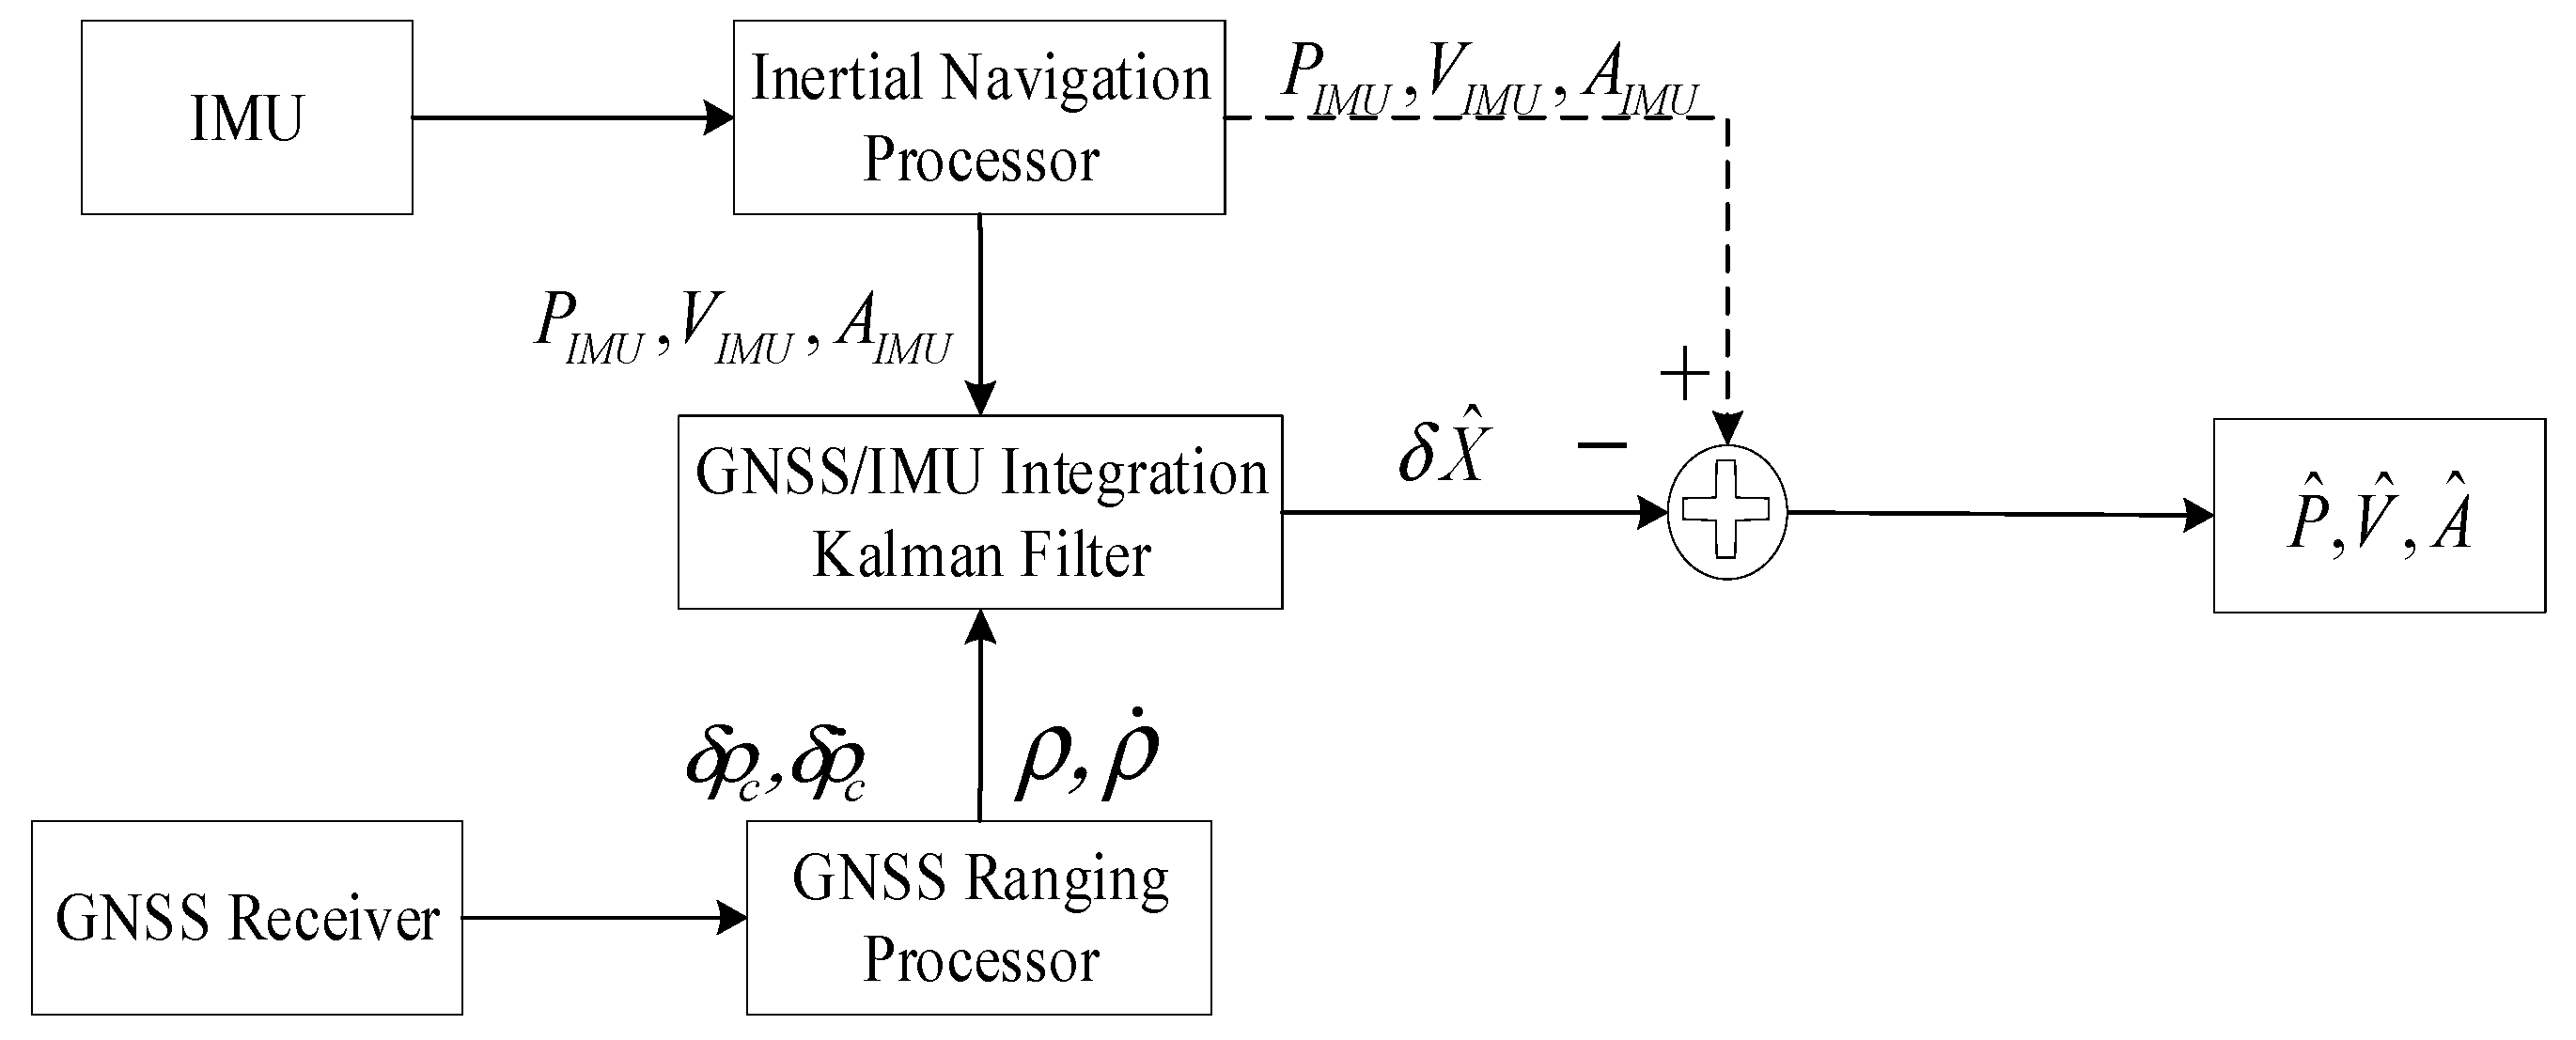
\includegraphics[width=1.0\linewidth]{Pictures/State_Estimation/Error_State_Kalman_Filter/Error_State_Kalman_Filter_Illustrated.png}
    \caption{Functional overview of the ESKF architecture. The filter propagates and estimates the small error state based on IMU data, updates it using GNSS measurements, and then injects the correction into the nominal state. After injection, the error state is reset to zero. This loop ensures stable and consistent estimation by combining fast IMU propagation with slower GNSS updates. Image taken from a paper on the Error State Kalman Filter.\textsuperscript{\cite{error_state_kalman_filter}}}
    \label{fig:state-estimation-error-state-kalman-filter}
\end{figure}

